\documentclass[../main.tex]{subfiles}
\graphicspath{
    {"../img/"}
    {"img/"}
}

\begin{document}
    Widzimy, że ten obrazek, który nam się jawi jest w miarę rozbudowany.
    Ostatnio wprowadziliśmy na baloniku układ współrzędnych.\\
    \begin{align*}
        &v = [\sigma], v\in T_pM, v\left(  \right) \in D_pM\\
        &v(f) = \frac{d}{dt}f(\sigma(t))|_{t=0} \\
        &v\left(  \right) = ?\cdot ? + ?\cdot ? + ?\cdot ? = \frac{d}{dt}(f\circ \varphi^{-1} \circ \varphi \circ \sigma(t))|_{t=0}=\\
        &= \frac{d}{dt}(\tilde f\circ \varphi(\sigma(t)))|_{t=0} = \frac{d}{dt}(\tilde f(\varphi^1(\sigma(t)),\varphi^2(\sigma(t)),\ldots,\varphi^n(\sigma(t))))|_{t=0}= \\
        &= \frac{\partial \tilde f}{\partial x^1} \frac{\partial \varphi^1(\sigma(t))}{\partial t} +\ldots+\frac{\partial \tilde f}{\partial x^n} \frac{\partial \varphi^n(\sigma(t))}{\partial t}
    .\end{align*}
    Czyli jeżeli $v\in T_pM$ i $v\in[\sigma]$, to wiemy, że
    \begin{align*}
        &v = \frac{\partial \varphi^1(\sigma(t))}{\partial t}|_{t=0} e_1 + \frac{\partial \varphi^2(\sigma(t))}{\partial t}|_{t=0} e_2 + \ldots + \frac{\partial \varphi^n(\sigma(t))}{\partial t}|_{t=0} e_n= \\
        &= \xi^1e_1 + \xi^2e_2 + \ldots + \xi^ne_n = \\
        &= \xi_1 \frac{\partial \tilde f}{\partial x^1} + \xi_2 \frac{\partial \tilde f}{\partial x^2} +\ldots+ \xi_n \frac{\partial \tilde f}{\partial x^n} = v(f)
    .\end{align*}
    Zatem \[
        v\left(  \right) = \xi_1 \frac{\partial }{\partial x^1} + \xi_2 \frac{\partial }{\partial x^2}  + \ldots + \xi_n \frac{\partial }{\partial x^n}
    .\]
    \begin{przyklad}
        Więc niech $v = 2e_x + 3e_y \to v\left(  \right) = 2 \cdot \frac{\partial }{\partial x} + 3 \cdot \frac{\partial }{\partial y} $.
    \end{przyklad}
    Wniosek: mając izomorfizm między $T_pM$ i $D_pM$ możemy zapisać bazy:
    \[
    T_pM = \left<e_1,e_2,\ldots,e_n \right>
    .\]
    To wtedy
    \[
    D_pM = \left<\frac{\partial }{\partial x^1} , \frac{\partial }{\partial x^2} ,\ldots,\frac{\partial }{\partial x^n}  \right>
    .\]
    np. $v = 7 e_r + 8 e_\varphi \to v\left(  \right) = 7 \frac{\partial }{\partial r} + 8 \frac{\partial }{\partial \varphi} $ (często użyjemy bazy z $D_pM$ jako bazy $T_pM$ ).
    \begin{definicja}
        Wektorem kostycznym (albo jednoformą) nazywamy odwzorowanie liniowe  $\omega: T_pM\to\mathbb{R}$.
        Zbiór jednoform ($p\in M$) oznaczamy przez $T_p^* M$ (lub $\Lambda^1(M)$, $\Lambda^1(\theta), \theta\in M$)
    \end{definicja}
    Skoro $T_p^* M$ jest dualna do $T_pM$, to ma ten sam wymiar i możemy wprowadzić bazę dualną. $T_p^*M = \left< dx^1, dx^2, \ldots, dx^n \right>$, gdzie $\left<dx^i, \frac{\partial }{\partial x^i}  \right> = \delta^i_j$
    \begin{przyklad}
        Niech $\Lambda^1(M)\to\omega = 7dx + 3dy, v\in T_pM = 2 \frac{\partial }{\partial x} +4 \frac{\partial }{\partial y} $, wówczas
        \begin{align*}
            &\left<\omega,v \right> = \left<7dx+3dy,2 \frac{\partial }{\partial x} + 4 \frac{\partial }{\partial y}  \right> =\\
            &= \left<7dx, 2 \frac{\partial }{\partial x} + 4 \frac{\partial }{\partial y}  \right> + 3 \left< dy, 2 \frac{\partial }{\partial x} + 4 \frac{\partial }{\partial y}  \right> = \\
            &= 7\cdot 2\left<dx,\frac{\partial }{\partial x}  \right> + 7\cdot 4 \left<dx, \frac{\partial }{\partial y}  \right> + 3\cdot 2 \left<dy,\frac{\partial }{\partial x}\right> + 3\cdot 4 \left<dy , \frac{\partial }{\partial y} \right> \\
            &= 7\cdot 2+ 3\cdot 4
        .\end{align*}
    \end{przyklad}
    \begin{przyklad}
        \begin{align*}
            &v = A^x \frac{\partial }{\partial x} + A^y \frac{\partial }{\partial y} + A^z \frac{\partial }{\partial z} , \omega = B_xdx + B_ydy + B_zdz=\\
            &= \left<\omega,v \right> = A^xB_x + A^yB_y + A^zB_z
        .\end{align*}
    \end{przyklad}
    \begin{figure}
        \centering
        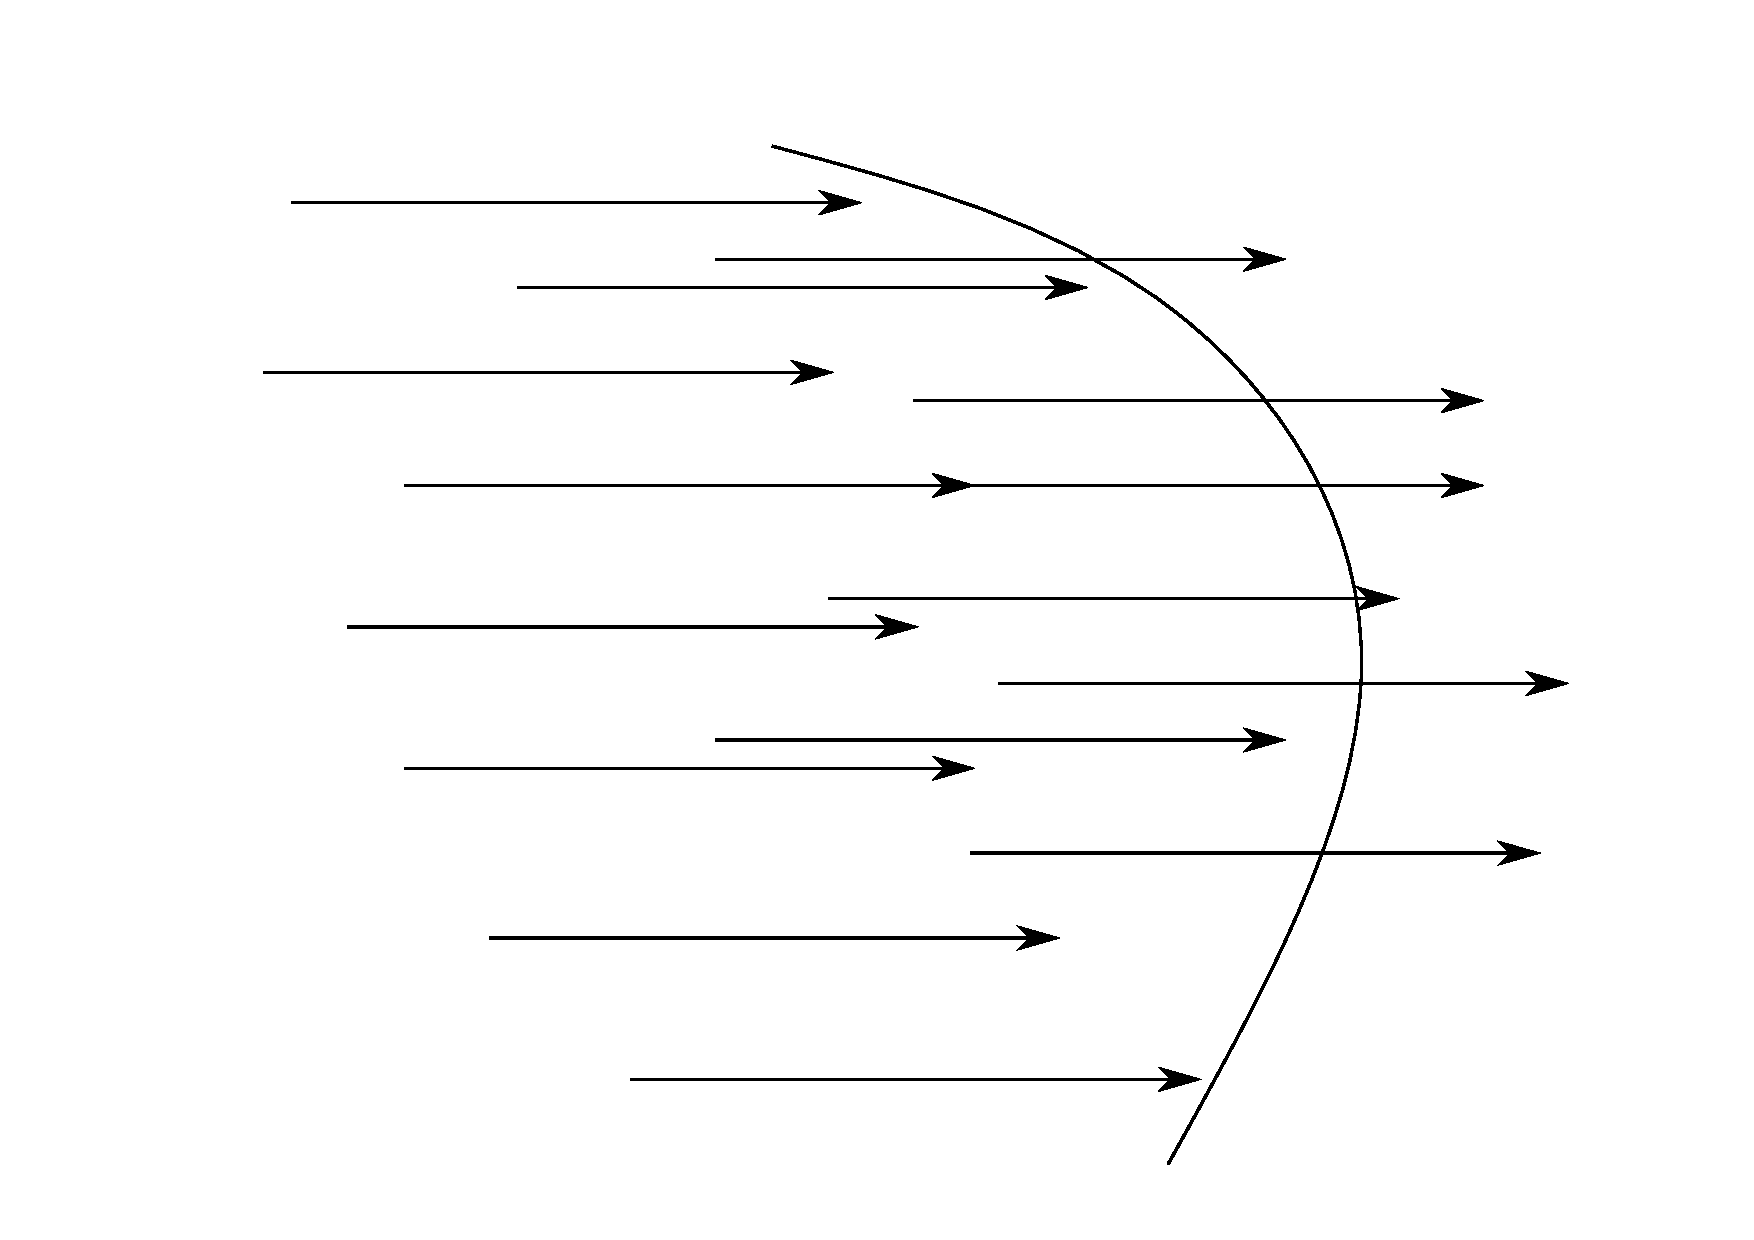
\includegraphics[width=\textwidth]{fig_50}
        \caption{Strumień przez balonik}
    \end{figure}

    \pagebreak
    \begin{definicja}
        Zbiór wszystkich odwzorowań $T_pM \times \ldots \times T_pM \to \mathbb{R}$ k - liniowych w każdej zmiennej i antysymetrycznych oznaczamy przez $\Lambda^k(M)$ i nazywamy k-formami.
    \end{definicja}
    \begin{definicja}
        Niech $\alpha\in T_p^*M, \beta\in T_p^*M ( \alpha\in \Lambda_p^1 M, \beta \in \Lambda_p^1 M )$.\\
        Odwzorowanie $\land : T_p^* M \times T_p^* M \to \Lambda^2(\theta), \theta\in M$ nazywamy iloczynem zewnętrznym i definiujemy tak:
        \[
            \left<\alpha\land\beta;v,w \right> \overset{\text{def}}{=} \begin{vmatrix}\alpha(v)&\beta(v)\\ \alpha(w)&\beta(w) \end{vmatrix}
        .\]
    \end{definicja}

    \begin{przyklad}
        Niech $\alpha = 7dx + 4dy, \beta = 2dx+3dy, v = 1 \frac{\partial }{\partial x} + 4 \frac{\partial }{\partial y} , w = 2 \frac{\partial }{\partial x} + \frac{\partial }{\partial y}$\\
        Wtedy
        \[
            \left<\alpha\land\beta;v,w \right> = \begin{vmatrix}\alpha(v)&\beta(v)\\ \alpha(w)&\beta(w)\end{vmatrix} = \begin{vmatrix}7\cdot 1+4\cdot 4& 2\cdot 1+3\cdot 4 \\ 7\cdot 2+4 & 2\cdot 2+3 \end{vmatrix}
        .\]
    \end{przyklad}
    Obserwacja: $\alpha\land\beta = -\beta\land\alpha$. Tzn. $\alpha\land\alpha = 0$.
    Ważny przykład:
    \begin{przyklad}
        \begin{align*}
            &\alpha = A_xdx + A_ydy + A_zdz, \beta = B_xdx + B_ydy + B_zdz\\
            & \alpha\land\beta = \left( A_xdx + A_ydy + A_zdz \right) \land \left( B_xdx + B_ydy + B_zdz \right) = \\
            &= \left( A_xdx+A_ydy+A_zdz \right) \land B_xdx + \left( A_xdx+A_ydy+A_zdz \right) \land B_ydy + \\
            &+ \left( A_xdx+A_ydy+A_zdz \right) \land B_zdz = A_yB_xdy\land dx + A_zB_x dz\land dx +   \\
            &+ A_xB_y dx\land dy + A_zB_ydz\land dy + A_xB_zdx\land dz + A_yB_zdy\land dz = \\
            &=  \left( A_xB_y - A_yB_x \right) dx\land dy + \left( A_yB_z - A_zB_y \right) dy\land dz + \left( A_zB_x - A_xB_z \right) dz\land dx\\
        .\end{align*}
    \end{przyklad}
    Potrzebujemy jeszcze jednego klocka, żeby zobaczyć gdzie tu siedzi fizyka.
    \begin{definicja}
        Odwzorowanie $d: \Lambda^k(M)\to\Lambda^{k+1}(M)$ nazywamy różniczką zewnętrzną (ewentualnie pochodną zewnętrzną) i definiujemy następująco:
        \begin{align*}
            &df = \frac{\partial f}{\partial x^1} dx^1 + \frac{\partial f}{\partial x^2} dx^2 + \ldots + \frac{\partial f}{\partial x^n} dx^n, f: \theta \to \mathbb{R}\\
            &(\text{funkcje nazywamy zero-formami }f\in \Lambda^0(\theta))\\
            &\omega\in\Lambda^p(\theta), \eta\in \Lambda^L(\theta) \implies d(\omega\land\eta) = d\omega\land\eta + (-1)^p\omega\land d\eta \\
            &dd\omega = 0, \omega\in\Lambda^k(\theta)
        .\end{align*}
    \end{definicja}
    \begin{przyklad}
        $f(r,\theta,\varphi)$ - funkcja z $\mathbb{R}^3$ w $\mathbb{R}^1$.\\
        \begin{align*}
            &df = \frac{\partial f}{\partial r} dr + \frac{\partial f}{\partial \theta} d\theta + \frac{\partial f}{\partial \varphi} d\varphi\\
            &\alpha = 7x^2y dx\\
            &d\alpha = d(7x^2y)\land dx = \left( \frac{\partial }{\partial x} (7x^2y)dx + \frac{\partial }{\partial y} (7x^2y)dy \right) \land dx = 7x^2dy\land dx
        .\end{align*}
    \end{przyklad}
    \begin{przyklad}
        Niech $F = -E_xdt\land dx - E_xdt\land dy - E_z dt\land dz + B_xdy\land dz + B_y dz\land dx + B_zdx \land dy$
        \begin{align*}
            &dF = \left( -\frac{\partial E_x}{\partial y} dy - \frac{\partial E_x}{\partial z} dz \right) \land dt\land dx +\\
            &+ \left( - \frac{\partial E_y}{\partial x}dx - \frac{\partial E_y}{\partial z}dz  \right)\land dt \land dy + \\
            &+ \left( -\frac{\partial E_z}{\partial x} dx - \frac{\partial E_z}{\partial y} dy \right)\land dt \land dz + \\
            &+ \left( \frac{\partial B_x}{\partial t} dt + \frac{\partial B_x}{\partial x} dx \right) \land dy \land dz + \\
            &+ \left( \frac{\partial B_y}{\partial t} dt + \frac{\partial B_y}{\partial y} dy \right) \land dz \land dx + \\
            &+ \left( \frac{\partial B_z}{\partial t} dt + \frac{\partial B_z}{\partial z} dz \right) \land dx \land dy = \\
            &= \underbrace{\left( -\frac{\partial E_x}{\partial y} + \frac{\partial E_y}{\partial x} + \frac{\partial B_z}{\partial t}  \right)} dt\land dx\land dy + \\
            &+ \underbrace{\left( -\frac{\partial E_y}{\partial z} + \frac{\partial E_z}{\partial y} + \frac{\partial B_x}{\partial t}  \right)} dt\land dy\land dz + \\
            &+ \underbrace{\left( -\frac{\partial E_x}{\partial z} + \frac{\partial E_z}{\partial x} - \frac{\partial B_y}{\partial t}  \right)}_{rot E - \frac{\partial B}{\partial t} } dt\land dx\land dz + \\
            &+ \underbrace{\left( \frac{\partial B_x}{\partial x} + \frac{\partial B_y}{\partial y} + \frac{\partial B_z}{\partial z}  \right)}_{\nabla B} dx\land dy\land dz
        .\end{align*}
        I to są równania Maxwella (przynajmniej pierwsza ich część) $dF = 0$
    \end{przyklad}


\end{document}
